\subsection{Late Fusion}

\begin{frame}[allowframebreaks]{Late Fusion: Overview}
    \begin{itemize}
        \item \textbf{Process frames separately}, then combine their representations.
        \item \textbf{Fully Connected Fusion}: Concatenate frame features, then use fully connected (FC) layers.
        \item \textbf{Pooling Fusion}: Apply average or max pooling across time dimension.
    \end{itemize}
    \vspace{1em}
    \textbf{Pros:} Simple and easy to implement.\\
    \textbf{Cons:} Weak temporal modeling; ignores complex temporal dependencies.
\end{frame}

\begin{frame}[allowframebreaks]{Late Fusion (with FC layers)}
    \begin{figure}
        \centering
        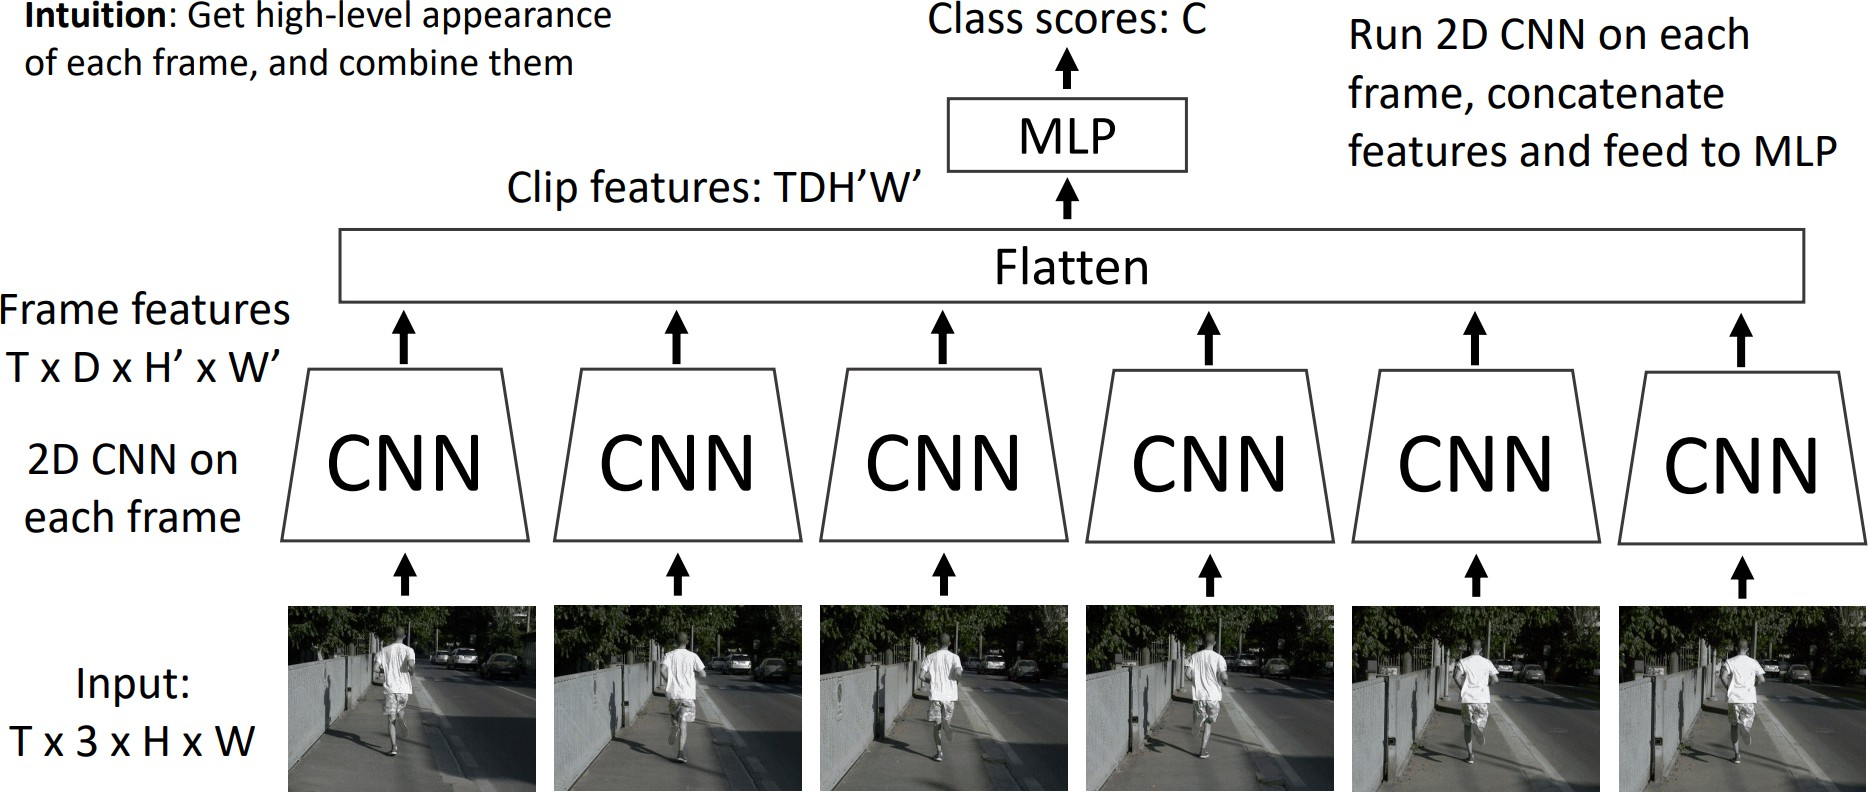
\includegraphics[width=1\textwidth,height=0.9\textheight,keepaspectratio]{images/video/slide_10_1_img.jpg}
    \end{figure}
\end{frame}

\begin{frame}[allowframebreaks]{Late Fusion (with pooling)}
    \begin{figure}
        \centering
        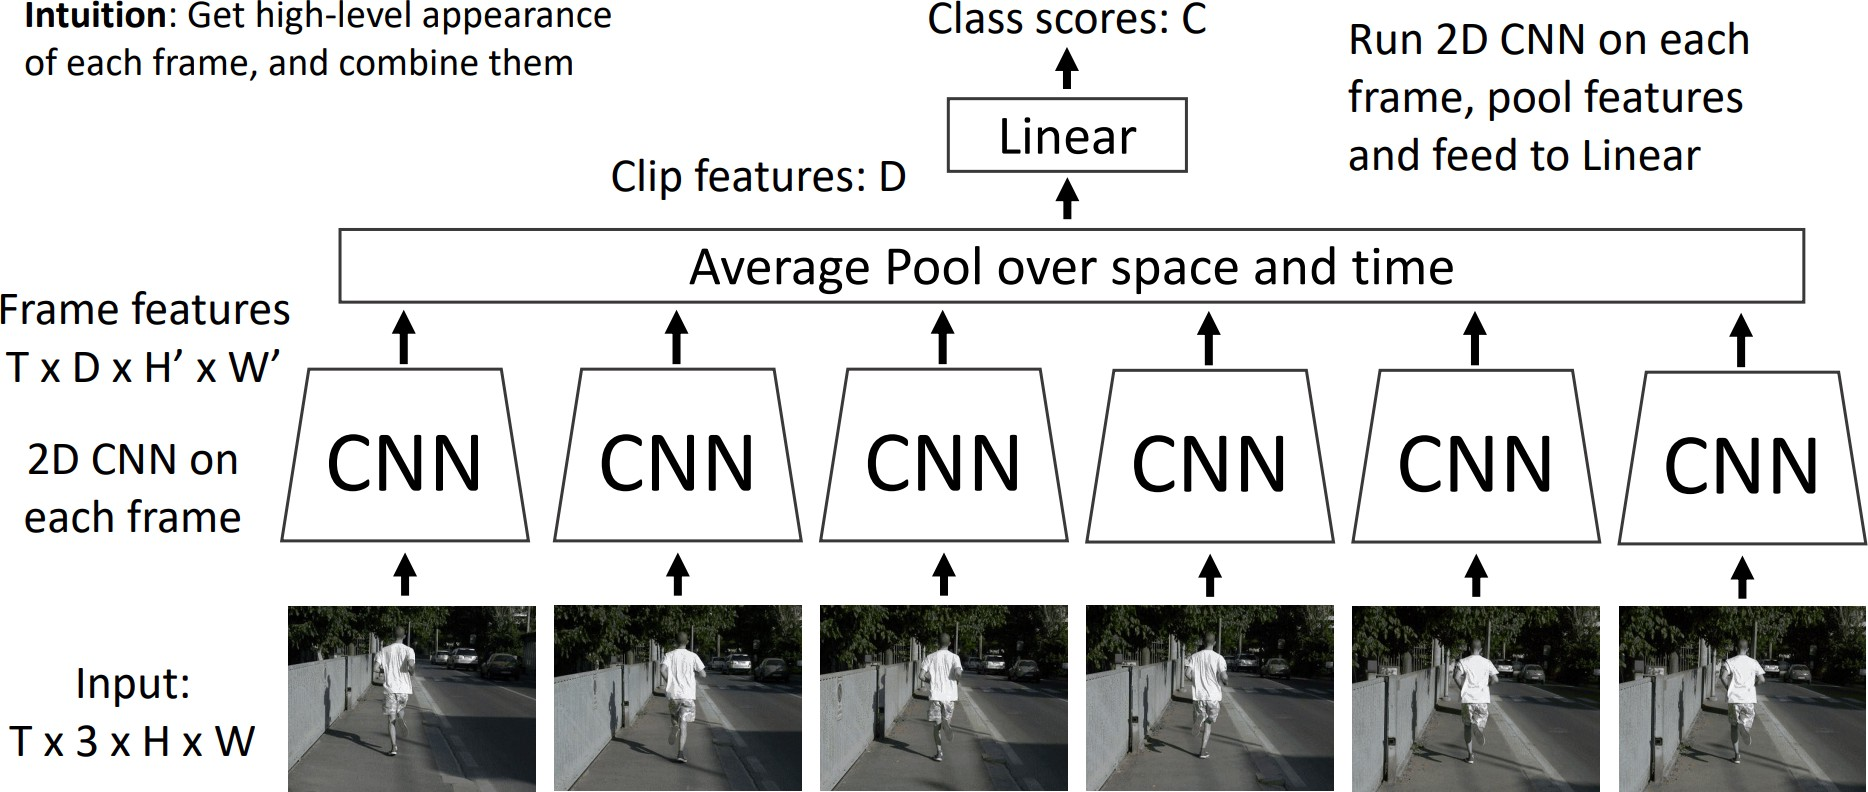
\includegraphics[width=1\textwidth,height=0.9\textheight,keepaspectratio]{images/video/slide_11_1_img.jpg}
    \end{figure}
\framebreak
    \begin{figure}
        \centering
        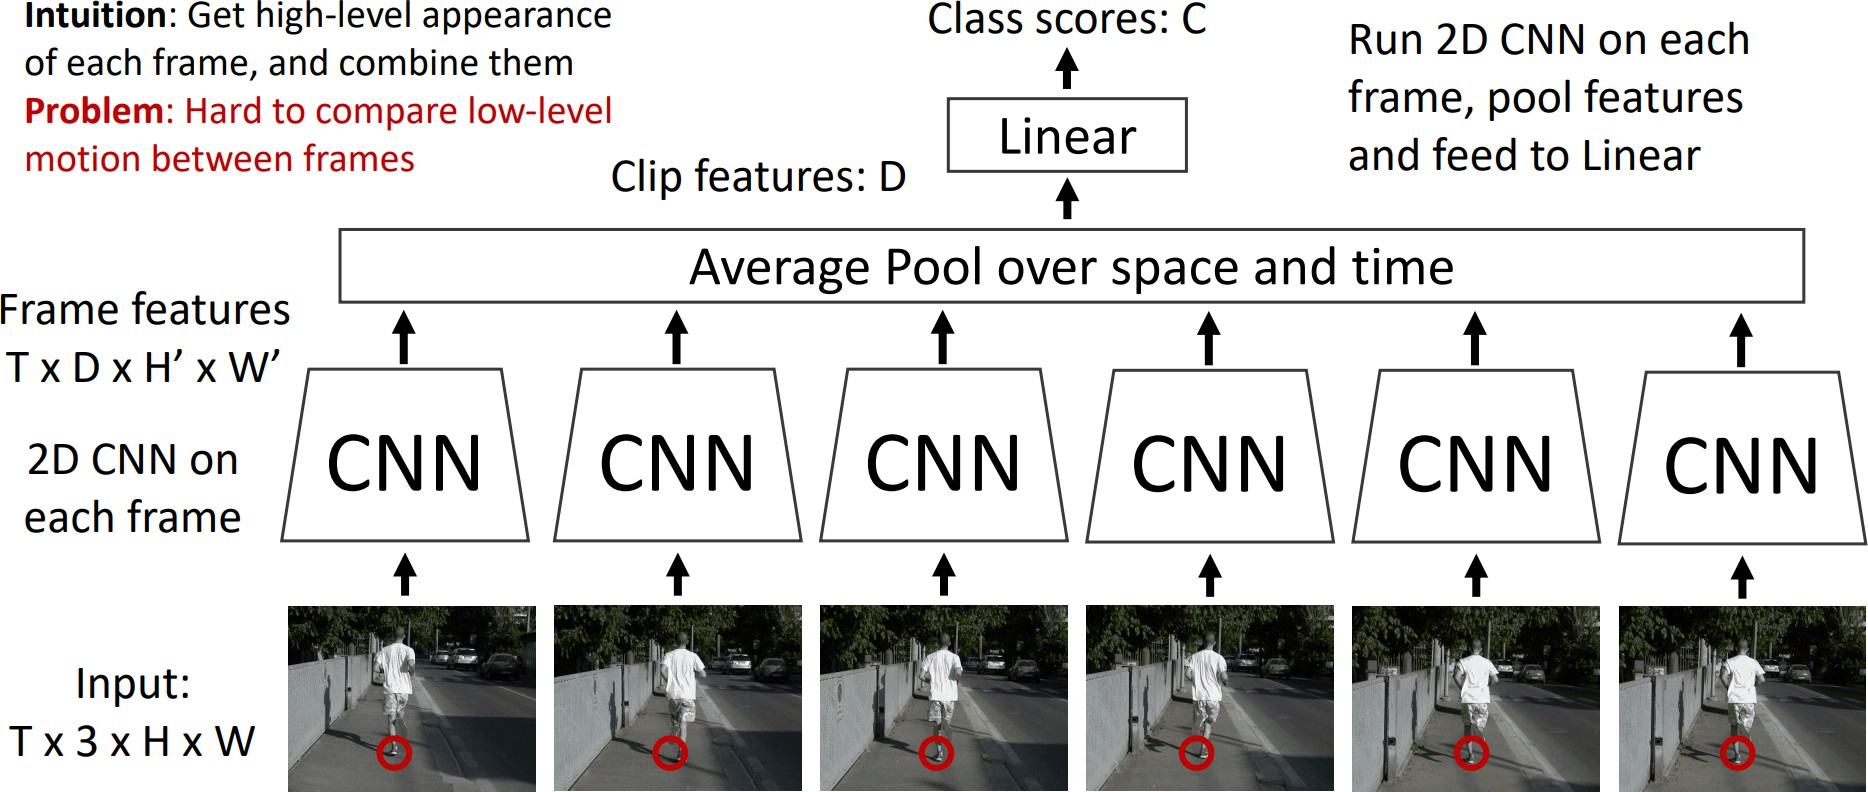
\includegraphics[width=1\textwidth,height=0.9\textheight,keepaspectratio]{images/video/slide_12_1_img.jpg}
    \end{figure}
\end{frame}